% 若编译失败,且生成 .synctex(busy) 辅助文件,可能有两个原因:
% 1. 需要插入的图片不存在:Ctrl + F 搜索 'figure' 将这些代码注释/删除掉即可
% 2. 路径/文件名含中文或空格:更改路径/文件名即可

% --------------------- 文章宏包及相关设置 --------------------- %
% >> ------------------ 文章宏包及相关设置 ------------------ << %
% 设定文章类型与编码格式
\documentclass[UTF8]{report}		

% 自定义宏定义
    \def\N{\mathbb{N}}
    \def\F{\mathbb{F}}
    \def\Z{\mathbb{Z}}
    \def\Q{\mathbb{Q}}
    \def\R{\mathbb{R}}
    \def\C{\mathbb{C}}
    \def\T{\mathbb{T}}
    \def\S{\mathbb{S}}
    \def\A{\mathbb{A}}
    \def\I{\mathscr{I}}
    \def\Im{\mathrm{Im\,}}
    \def\Re{\mathrm{Re\,}}
    \def\d{\mathrm{d}}
    \def\p{\partial}

% 导入基本宏包
    \usepackage[UTF8]{ctex}     % 设置文档为中文语言
    \usepackage[colorlinks, linkcolor=blue, anchorcolor=blue, citecolor=blue, urlcolor=blue]{hyperref}  % 宏包:自动生成超链接 (此宏包与标题中的数学环境冲突)
    % \usepackage{docmute}    % 宏包:子文件导入时自动去除导言区,用于主/子文件的写作方式,\include{./51单片机笔记}即可。注:启用此宏包会导致.tex文件capacity受限。
    \usepackage{amsmath}    % 宏包:数学公式
    \usepackage{mathrsfs}   % 宏包:提供更多数学符号
    \usepackage{amssymb}    % 宏包:提供更多数学符号
    \usepackage{pifont}     % 宏包:提供了特殊符号和字体
    \usepackage{extarrows}  % 宏包:更多箭头符号


% 文章页面margin设置
    \usepackage[a4paper]{geometry}
        \geometry{top=1in}
        \geometry{bottom=1in}
        \geometry{left=0.75in}
        \geometry{right=0.75in}   % 设置上下左右页边距
        \geometry{marginparwidth=1.75cm}    % 设置边注距离(注释、标记等)

% 配置数学环境
    \usepackage{amsthm} % 宏包:数学环境配置
    % theorem-line 环境自定义
        \newtheoremstyle{MyLineTheoremStyle}% <name>
            {11pt}% <space above>
            {11pt}% <space below>
            {}% <body font> 使用默认正文字体
            {}% <indent amount>
            {\bfseries}% <theorem head font> 设置标题项为加粗
            {:}% <punctuation after theorem head>
            {.5em}% <space after theorem head>
            {\textbf{#1}\thmnumber{#2}\ \ (\,\textbf{#3}\,)}% 设置标题内容顺序
        \theoremstyle{MyLineTheoremStyle} % 应用自定义的定理样式
        \newtheorem{LineTheorem}{Theorem.\,}
    % theorem-block 环境自定义
        \newtheoremstyle{MyBlockTheoremStyle}% <name>
            {11pt}% <space above>
            {11pt}% <space below>
            {}% <body font> 使用默认正文字体
            {}% <indent amount>
            {\bfseries}% <theorem head font> 设置标题项为加粗
            {:\\ \indent}% <punctuation after theorem head>
            {.5em}% <space after theorem head>
            {\textbf{#1}\thmnumber{#2}\ \ (\,\textbf{#3}\,)}% 设置标题内容顺序
        \theoremstyle{MyBlockTheoremStyle} % 应用自定义的定理样式
        \newtheorem{BlockTheorem}[LineTheorem]{Theorem.\,} % 使用 LineTheorem 的计数器
    % definition 环境自定义
        \newtheoremstyle{MySubsubsectionStyle}% <name>
            {11pt}% <space above>
            {11pt}% <space below>
            {}% <body font> 使用默认正文字体
            {}% <indent amount>
            {\bfseries}% <theorem head font> 设置标题项为加粗
            {:\\ \indent}% <punctuation after theorem head>
            {0pt}% <space after theorem head>
            {\textbf{#3}}% 设置标题内容顺序
        \theoremstyle{MySubsubsectionStyle} % 应用自定义的定理样式
        \newtheorem{definition}{}

%宏包:有色文本框(proof环境)及其设置
    \usepackage[dvipsnames,svgnames]{xcolor}    %设置插入的文本框颜色
    \usepackage[strict]{changepage}     % 提供一个 adjustwidth 环境
    \usepackage{framed}     % 实现方框效果
        \definecolor{graybox_color}{rgb}{0.95,0.95,0.96} % 文本框颜色。修改此行中的 rgb 数值即可改变方框纹颜色,具体颜色的rgb数值可以在网站https://colordrop.io/ 中获得。(截止目前的尝试还没有成功过,感觉单位不一样)(找到喜欢的颜色,点击下方的小眼睛,找到rgb值,复制修改即可)
        \newenvironment{graybox}{%
        \def\FrameCommand{%
        \hspace{1pt}%
        {\color{gray}\small \vrule width 2pt}%
        {\color{graybox_color}\vrule width 4pt}%
        \colorbox{graybox_color}%
        }%
        \MakeFramed{\advance\hsize-\width\FrameRestore}%
        \noindent\hspace{-4.55pt}% disable indenting first paragraph
        \begin{adjustwidth}{}{7pt}%
        \vspace{2pt}\vspace{2pt}%
        }
        {%
        \vspace{2pt}\end{adjustwidth}\endMakeFramed%
        }

% 外源代码插入设置
    % matlab 代码插入设置
    \usepackage{matlab-prettifier}
        \lstset{
            style=Matlab-editor,  % 继承matlab代码颜色等
        }
    \usepackage[most]{tcolorbox} % 引入tcolorbox包 
    \usepackage{listings} % 引入listings包
        \tcbuselibrary{listings, skins, breakable}
        \lstdefinestyle{matlabstyle}{
            language=Matlab,
            basicstyle=\small,
            breakatwhitespace=false,
            breaklines=true,
            captionpos=b,
            keepspaces=true,
            numbers=left,
            numbersep=15pt,
            showspaces=false,
            showstringspaces=false,
            showtabs=false,
            tabsize=2
        }
        \newtcblisting{matlablisting}{
            arc=3pt,        % 圆角半径
            top=-5pt,
            bottom=-5pt,
            left=1mm,
            listing only,
            listing style=matlabstyle,
            breakable,
            colback=white   % 选一个合适的颜色
        }

% table 支持
    \usepackage{booktabs}   % 宏包:三线表
    \usepackage{tabularray} % 宏包:表格排版
    \usepackage{longtable}  % 宏包:长表格

% figure 设置
    \usepackage{graphicx}  % 支持 jpg, png, eps, pdf 图片 
    \usepackage{subcaption} % 支持子图
    \usepackage{svg}       % 支持 svg 图片
        \svgsetup{
            % 指向 inkscape.exe 的路径
            inkscapeexe = D:/aa_my_apps_main/Inkscape/bin/inkscape.exe, 
            % 一定程度上修复导入后图片文字溢出几何图形的问题
            inkscapelatex = false                 
        }

% 图表进阶设置
    \usepackage{caption}    % 图注、表注
        \captionsetup[figure]{name=图}  
        \captionsetup[table]{name=表}
        \captionsetup{labelfont=bf, font=small}
    \usepackage{float}     % 图表位置浮动设置 

% 圆圈序号自定义
    \newcommand*\circled[1]{\tikz[baseline=(char.base)]{\node[shape=circle,draw,inner sep=0.8pt, line width = 0.03em] (char) {\small \bfseries #1};}}   % TikZ solution

% 列表设置
\usepackage{enumitem}   % 宏包:列表环境设置
    \setlist[enumerate]{
        label=\bfseries(\arabic*) ,   % 设置序号样式为加粗的 (1) (2) (3)
        ref=\arabic*, % 如果需要引用列表项,这将决定引用格式(这里仍然使用数字)
        itemsep=0pt, parsep=0pt, topsep=0pt, partopsep=0pt, leftmargin=3.5em} 
    \setlist[itemize]{itemsep=0pt, parsep=0pt, topsep=0pt, partopsep=0pt, leftmargin=3.5em}
    \newlist{circledenum}{enumerate}{1} % 创建一个新的枚举环境  
    \setlist[circledenum,1]{  
        label=\protect\circled{\arabic*}, % 使用 \arabic* 来获取当前枚举计数器的值,并用 \circled 包装它  
        ref=\arabic*, % 如果需要引用列表项,这将决定引用格式(这里仍然使用数字)
        itemsep=0pt, parsep=0pt, topsep=0pt, partopsep=0pt, leftmargin=3.5em
    }  
    

% 其它设置
    % 脚注设置
    \renewcommand\thefootnote{\ding{\numexpr171+\value{footnote}}}
    % 参考文献引用设置
        \bibliographystyle{unsrt}   % 设置参考文献引用格式为unsrt
        \newcommand{\upcite}[1]{\textsuperscript{\cite{#1}}}     % 自定义上角标式引用
    % 文章序言设置
        \newcommand{\cnabstractname}{序言}
        \newenvironment{cnabstract}{%
            \par\Large
            \noindent\mbox{}\hfill{\bfseries \cnabstractname}\hfill\mbox{}\par
            \vskip 2.5ex
            }{\par\vskip 2.5ex}

% 文章默认字体设置
\usepackage{fontspec}   % 宏包:字体设置
    \setmainfont{SimSun}    % 设置中文字体为宋体字体
    \setmainfont{Times New Roman} % 设置英文字体为Times New Roman

% 各级标题自定义设置
    \usepackage{titlesec}   
    % chapter
        \titleformat{\chapter}[hang]{\normalfont\Large\bfseries\centering}{Homework \thechapter :}{10pt}{}
        \titlespacing*{\chapter}{0pt}{-30pt}{10pt} % 控制上方空白的大小
    % section
        \titleformat{\section}[hang]{\normalfont\large\bfseries}{\thesection}{8pt}{}
    % subsection
        %\titleformat{\subsubsection}[hang]{\normalfont\bfseries}{}{8pt}{}
    % subsubsection
        %\titleformat{\subsubsection}[hang]{\normalfont\bfseries}{}{8pt}{}

% --------------------- 文章宏包及相关设置 --------------------- %
% >> ------------------ 文章宏包及相关设置 ------------------ << %



% ------------------------ 文章信息区 ------------------------ %
% >> --------------------- 文章信息区 --------------------- << %
% 页眉页脚设置

\usepackage{fancyhdr}   %宏包:页眉页脚设置
    \pagestyle{fancy}
    \fancyhf{}
    \cfoot{\thepage}
    \renewcommand\headrulewidth{1pt}
    \renewcommand\footrulewidth{0pt}
    \chead{光学作业,\ 丁毅,\ 2023K8009908031}
    \lhead{Homework \thechapter}
    \rhead{dingyi233@mails.ucas.ac.cn}

%文档信息设置
\title{光学作业\\ Homework of Optics}
\author{丁毅\\ \footnotesize 中国科学院大学,北京 100049\\ Yi Ding \\ \footnotesize University of Chinese Academy of Sciences, Beijing 100049, China}
\date{\footnotesize 2024.9 -- 2025.1}
% >> --------------------- 文章信息区 --------------------- << %
% ------------------------ 文章信息区 ------------------------ %

% 开始编辑文章

\begin{document}
\zihao{5}           % 设置全文字号大小

% ------------------------ 封面序言与目录 ------------------------ %
% >> --------------------- 封面序言与目录 --------------------- << %
% 封面
    \maketitle\newpage  
    \pagenumbering{Roman} % 页码为大写罗马数字
    \thispagestyle{fancy}   % 显示页码、页眉等

% 序言
    \begin{cnabstract}\normalsize 
        本文为笔者本科时的“光学”课程作业(Homework of Optics, 2024.9-2025.1)。由于个人学识浅陋,认识有限,文中难免有不妥甚至错误之处,望读者不吝指正,在此感谢。\par 
        我的邮箱是 dingyi233@mails.ucas.ac.cn。
    \end{cnabstract}
    \addcontentsline{toc}{chapter}{序言} % 手动添加为目录

% 不换页目录
    \setcounter{tocdepth}{0}
    \noindent\rule{\textwidth}{0.1em}   % 分割线
    \noindent\begin{minipage}{\textwidth}\centering 
        \vspace{1cm}
        \tableofcontents\thispagestyle{fancy}   % 显示页码、页眉等   
    \end{minipage}  
    \addcontentsline{toc}{chapter}{目录} % 手动添加为目录

% 收尾工作
    \newpage    
    \pagenumbering{arabic} 

% >> --------------------- 封面序言与目录 --------------------- << %
% ------------------------ 封面序言与目录 ------------------------ %

\chapter{第一章}\thispagestyle{fancy}

\section{求入射到光纤的角度满足的条件}

\begin{equation}
    n_0 \sin i = n_g \sin i', \quad n_g \sin (\frac{\pi}{2} - i') = n_c \sin \frac{\pi}{2} 
     \Longrightarrow i \leqslant \arcsin 
\end{equation}
    

\begin{figure}[H]\centering
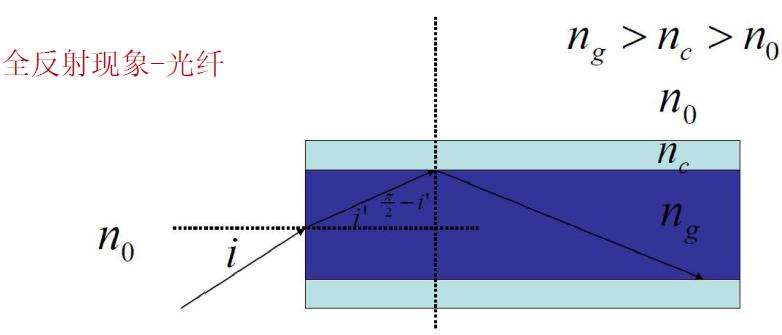
\includegraphics[width=0.55\textwidth]{assets/1/c6c9e6ef2f6755ead534508010ad0452 (2).jpg}
\caption{\textbf{求入射到光纤的角度满足的条件}}\label{求入射到光纤的角度满足的条件}
\end{figure}

\section{推导光线轨迹方程}

在 $x$-$y$ 平面中,设 $y = y(x)$ 表示光线的轨迹方程,$n = n(y)$ 表示介质的折射率。由几何关系,我们有:
\begin{equation}
\frac{\mathrm{d} y }{\mathrm{d} x } = \tan \theta = \frac{1}{\tan i} = \frac{\sqrt{1-\sin^2 i}}{\sin i} 
\end{equation}

由折射定律,记 $[n(y)\sin i(y)]_{y=0} = C$ ,则我们有:
\begin{equation}
n(y)\sin i(y) = C \Longrightarrow \frac{\mathrm{d} y }{\mathrm{d} x } = \frac{\sqrt{n^2 - C^2}}{C^2}, \quad \left(\frac{\mathrm{d} y }{\mathrm{d} x }\right)^{2} = \frac{n^2}{C^2} - 1
\end{equation}
两边同时对 $x$ 求导,得到:
\begin{equation}
2 \left(\frac{\mathrm{d} y }{\mathrm{d} x }\right) \left(\frac{\mathrm{d}^2 y }{\mathrm{d} x^2 }\right) = \frac{1}{C^2} \left(\frac{\mathrm{d} n^2 }{\mathrm{d} y }\right) \left(\frac{\mathrm{d} y }{\mathrm{d} x }\right) \Longrightarrow \frac{\mathrm{d}^2 y }{\mathrm{d} x^2 } = \frac{1}{2C^2}\cdot \frac{\mathrm{d} n^2 }{\mathrm{d} y } 
\end{equation}
也即
\begin{equation}
    \frac{\mathrm{d}^2 y }{\mathrm{d} x^2 } = \frac{1}{2n_0^2\sin^2 i}\cdot \frac{\mathrm{d} n^2 }{\mathrm{d} y } = \frac{1}{2n_0^2\cos^2 \theta}\cdot \frac{\mathrm{d} n^2 }{\mathrm{d} y } \quad 
\end{equation}
证毕。$\quad \square$

\begin{figure}[H]\centering
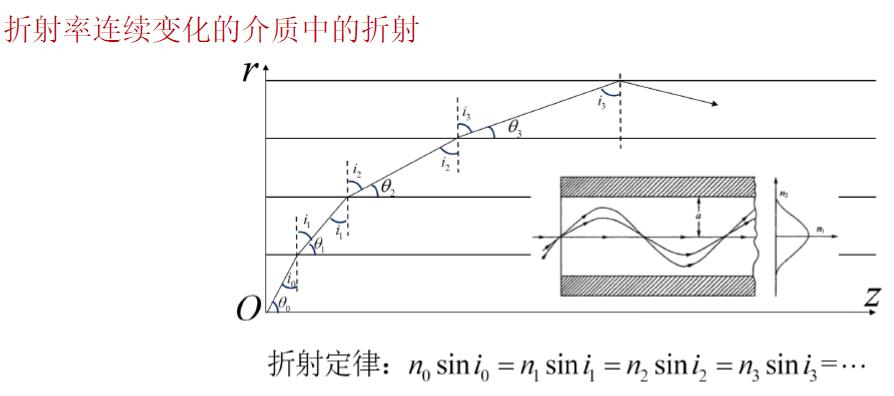
\includegraphics[width=0.8\textwidth]{assets/1/88b3f41951f9d3be9e2964935ebaf0f7.jpg}
\caption{\textbf{推导光线轨迹方程}}\label{推导光线轨迹方程}
\end{figure}

事实上,在三维坐标系中考虑上述过程,或者利用费马原理和变分法,又或考虑哈密顿光学,可以得到更一般的形式,称为光路方程,如下:
\begin{equation}
    \nabla n=\frac{\mathrm{d}}{\mathrm{d}s}\left(n\frac{\mathrm{d}\vec{r}}{\mathrm{d}s}\,\right)
\end{equation}

\section{(已被删去)}
\section{利用费马原理给出物像关系}

折射球面如图,由余弦定理可知:
\begin{equation}
\text{OPL} = np + n'p' 
= n \sqrt{r^2 + (s+r)^2 \,{\color{red} -}\, 2r(s+r)\cos \phi } + n' \sqrt{r^2 + (s'-r)^2 \,{\color{red} +}\, 2r(s'-r)\cos \phi } 
\end{equation}

由费马原理,$\frac{\mathrm{d} \text{OPL}  }{\mathrm{d} \phi } = 0$,于是有:
\begin{equation}
\frac{-nr(s+r)\sin \phi }{p} + \frac{n'r(s'-r)\sin \phi }{p'} = 0 \Longrightarrow  \frac{n}{p} + \frac{n'}{p'} = \frac{1}{R\,}\left( \frac{n's'}{p'} - \frac{ns}{p} \right)
\end{equation}

在傍轴条件下,有 $s \approx p$,$s' \approx p'$,于是有:
\begin{equation}
\frac{n}{s} + \frac{n'}{s'} = \frac{n' - n}{R}
\end{equation}
证毕。
\begin{figure}[H]\centering
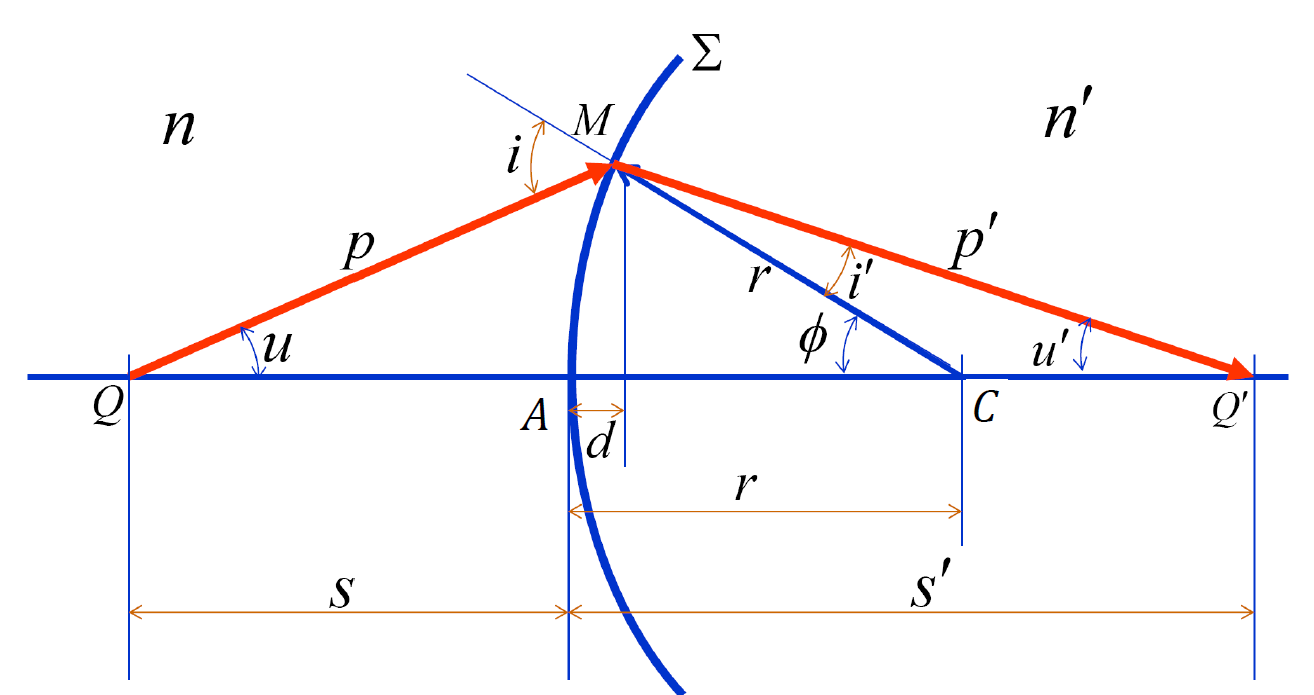
\includegraphics[width=0.45\textwidth]{assets/1/7dd67844c3c8000268c32546583de193.png}
\caption{\textbf{折射球面物像关系}}\label{折射球面物像关系}
\end{figure}

\section{推导反射球面的物像公式}

这里要注意,由于像是虚像,$l_2$ 贡献虚光程(为负),且 $s_2<0$,因此圆心到像点的距离为 $r+s_2$ 而非 $r-s_2$。同由余弦定理,写出光程 \text{OPL},有:
\begin{equation}
\text{OPL} = n_1l_1 - n_2l_2 
=
n_1\sqrt{r^2 + (r+s_1)^2 - 2r(r+s_1)\cos \phi } \,{\color{red} -}\, n_2 \sqrt{r^2 + (r+s_2)^2 - 2r(r+s_2)\cos \phi } 
\end{equation}

由费马原理,$\frac{\mathrm{d} \text{OPL}  }{\mathrm{d} \phi } = 0$,于是有:
\begin{equation}
\frac{-n_1r(r+s_1)\sin \phi }{l_1} + \frac{n_2r(r+s_2)\sin \phi }{l_2} = 0 
\Longrightarrow 
\frac{n_2}{l_2} - \frac{n_1}{l_1} = \frac{1}{r}\left( \frac{n_1s_1}{l_1} - \frac{n_2s_2}{l_2} \right)
\end{equation}
傍轴时,有 $s_1 \approx l_1$,$s_2 \approx -l_2$,于是:
\begin{equation}
-\frac{n_2}{l_2} - \frac{n_1}{l_1} = \frac{1}{r}(n_1 + n_2)
\end{equation}
当反射球面两侧为相同介质时,$n_1 = n_2$,则:
\begin{equation}
\frac{1}{s_1} + \frac{1}{s_2} = -\frac{2}{r}
\end{equation}
证毕。

\section{画出图中的像点}
如下图所示,左侧为手绘图,右侧为光路仿真软件 \href{https://www.optico.app/en/start-en/}{Optico} 效果图。

\begin{figure}[H]\centering
\begin{subfigure}[t]{0.47\textwidth}\centering
    \includegraphics[height=130pt]{assets/1/图1.png}
    \caption{\bfseries 手绘图 }
\end{subfigure}\begin{subfigure}[t]{0.52\textwidth}\centering
    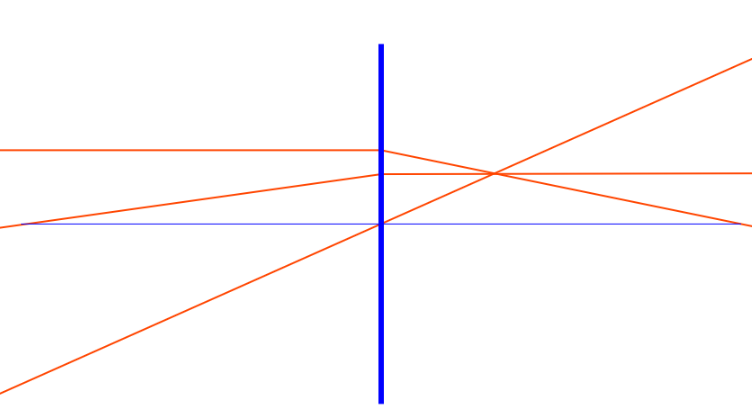
\includegraphics[height=130pt]{assets/1/1.png}
    \caption{\bfseries 光路仿真 }
\end{subfigure}
\caption{\bfseries 画出虚物 $Q$ 的像点 $Q'$}
\end{figure}

\begin{figure}[H]\centering
    \begin{subfigure}[t]{0.47\textwidth}\centering
        \includegraphics[height=130pt]{assets/1/图2.png}
        \caption{\bfseries 手绘图 }
    \end{subfigure}\begin{subfigure}[t]{0.52\textwidth}\centering
        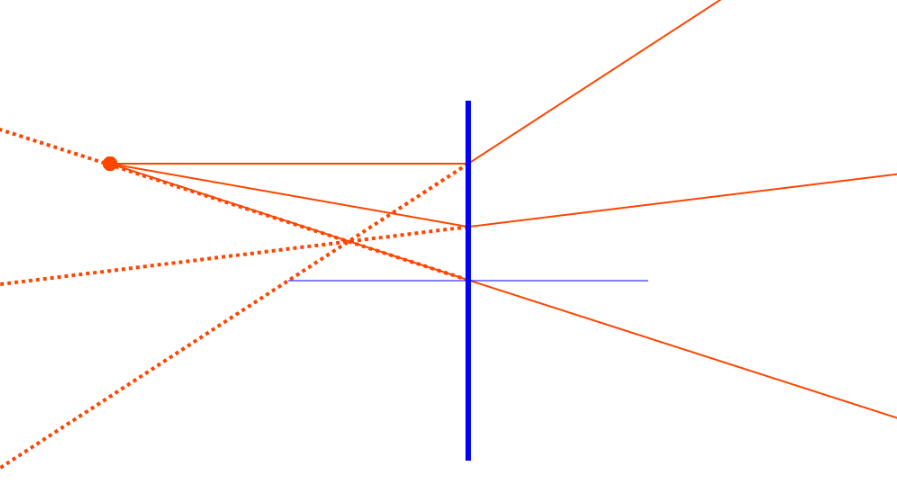
\includegraphics[height=130pt]{assets/1/2.png}
        \caption{\bfseries 光路仿真 }
    \end{subfigure}
    \caption{\bfseries 画出实物 $Q$ 经凹透镜的像点 $Q'$}
\end{figure}

    \begin{figure}[H]\centering
\begin{subfigure}[t]{0.47\textwidth}\centering
    \includegraphics[height=130pt]{assets/1/图3.png}
    \caption{\bfseries 手绘图 }
\end{subfigure}\begin{subfigure}[t]{0.52\textwidth}\centering
    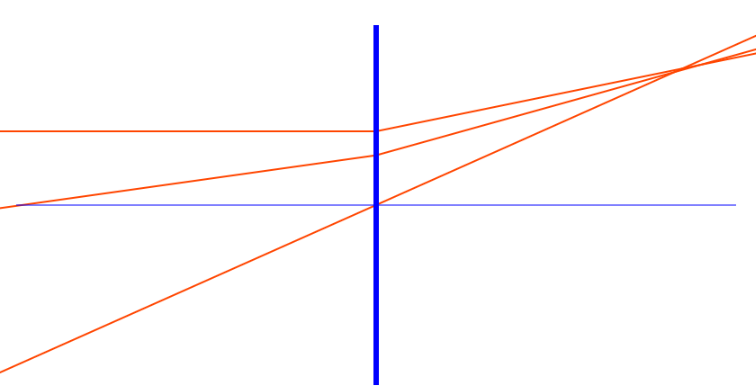
\includegraphics[height=130pt]{assets/1/3.png}
    \caption{\bfseries 光路仿真 }
\end{subfigure}
\caption{\bfseries 画出虚物 $Q$ 经凹透镜的像点 $Q'$}
\end{figure}



\chapter{第二章}\thispagestyle{fancy}

\section{对于正入射的情况,写出菲涅尔公式}

菲涅尔公式如下:

\begin{table}[H]
    \centering
    \begin{tabular}{|c|c|c|c|c|} 
    \hline
    类型 & \multicolumn{2}{c|}{振幅反射系数 $r$} & \multicolumn{2}{c|}{振幅透射系数 $t$ }  \\ 
    \hline
    s 波 & $\displaystyle r_s = \frac{n_i\cos \theta_i - n_t \cos \theta_t}{n_i\cos \theta_i + n_t \cos \theta_t} $ & $\displaystyle  - \frac{\sin (\theta_i - \theta_t) }{\sin (\theta_i + \theta_t)}$ & $\displaystyle t_s  = \frac{2n_i \cos \theta_i}{n_i\cos \theta_i + n_t \cos \theta_t} $ &   $\displaystyle  + \frac{2 \sin \theta_t \cos \theta_i}{\sin (\theta_i + \theta_t)}$   \\ 
    \hline
    p 波 & $\displaystyle r_p = \frac{n_t\cos \theta_i - n_i \cos \theta_t}{n_t\cos \theta_i + n_i \cos \theta_t} $ &     $ \displaystyle  + \frac{\tan (\theta_i - \theta_t)}{\tan (\theta_i + \theta_t)} $  &  $\displaystyle t_p  = \frac{2n_i \cos \theta_i}{n_i\cos \theta_t + n_t \cos \theta_i} $ &   $\displaystyle + \frac{2 \sin \theta_t \cos \theta_i}{\sin (\theta_i + \theta_t) \cos (\theta_i - \theta_t)}$                  \\
    \hline
    \end{tabular}
\end{table}

正入射时,$\theta_i = \theta_t = 0$,于是有:
\begin{gather}
    r_p = (-r_s)  = \frac{n_t - n_i}{n_t + n_i},\quad t_p = t_s = \frac{2n_i}{n_i + n_t} \\ 
    F = R_s = R_p = \left( \frac{n_t - n_i}{n_t + n_i} \right)^2
\end{gather}


不妨作出相关的图像,图 \ref{振幅系数随入射角的变化} 是 s 波、p 波振幅系数关于入射角 $\theta_i$ 的变化情况\footnote{源码见附录 \ref{图振幅系数随入射角的变化源码}}。

\begin{figure}[H]\centering
\begin{subfigure}[t]{0.49\textwidth}\centering
    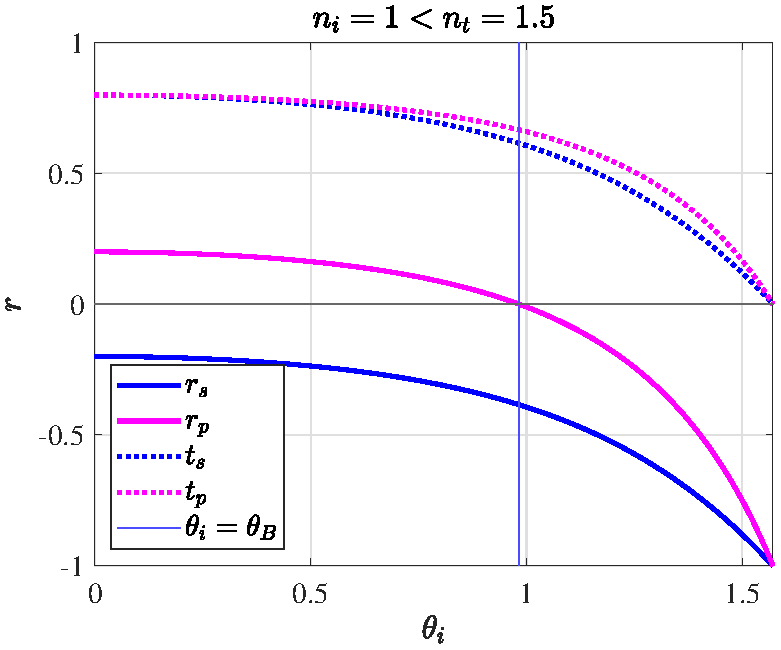
\includegraphics[height=180pt]{assets/2/2024-09-15_10-53-31.pdf}
    \caption{\bfseries 由空气入射玻璃($n_i = 1,\ n_t = 1.5$) }
\end{subfigure}
\begin{subfigure}[t]{0.49\textwidth}\centering
    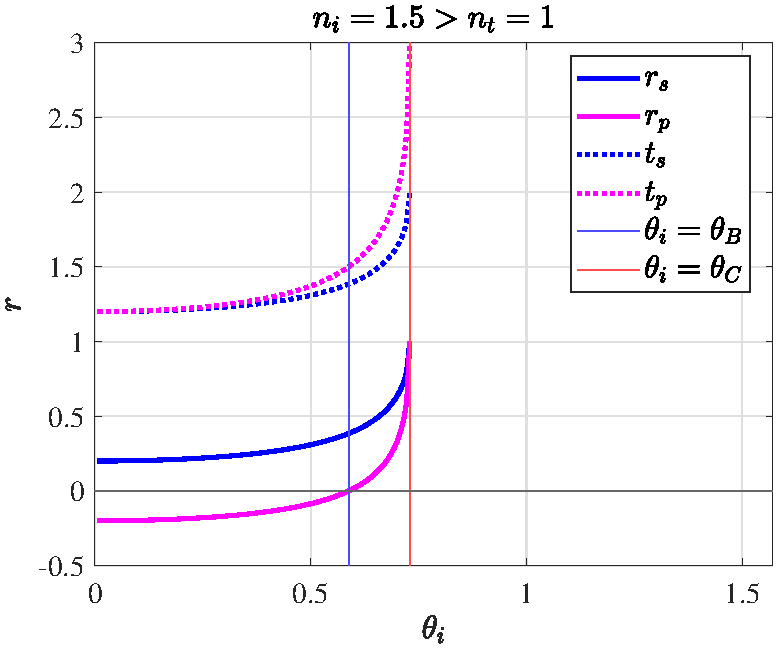
\includegraphics[height=180pt]{assets/2/2024-09-15_10-53-27.pdf}
    \caption{\bfseries 由玻璃入射空气($n_i = 1.5,\ n_t = 1$) }
\end{subfigure}
\caption{\bfseries 振幅系数 $r$ 随入射角 $\theta_i$ 的变化 }\label{振幅系数随入射角的变化}
\end{figure}


\section{一自然光以 Brewster Angle 入射到空气中的一块玻璃,已知功率透射率为 0.86。}
\begin{enumerate}
\item \textbf{求功率的反射率:}

$T = 0.86$,由能量守恒,功率反射率 $R = 0.14$。
\item \textbf{若输入为 1000 W,求透射光 s 分量上的功率}

光束为自然光,因此 s 分量和 p 分量的功率相同,都为 500 W。先求解入射角 $\theta_i$,由菲涅尔定理和能量关系:
\begin{equation}
R =  \frac{1}{2}(R_s + R_p),\  R_s =  \left[ \frac{ \cos \theta_i - \sqrt{n_{ti}^2 - \sin^2 \theta_i} }{\cos \theta_i + \sqrt{n_{ti}^2 - \sin^2 \theta_i}} \right]^2,\ R_p = \left[ \frac{ n_{ti}^2\cos \theta_i - \sqrt{n_{ti}^2 - \sin^2 \theta_i} }{n_{ti}^2\cos \theta_i + \sqrt{n_{ti}^2 - \sin^2 \theta_i}} \right]^2
\end{equation}
其中 $n_i = 1$,$n_t = 1.5$,因此 $n_{ti} = 1.5$,代入即得:
\begin{equation}
    \left[ \frac{ \cos \theta_i - \sqrt{1.5^2 - \sin^2 \theta_i} }{\cos \theta_i + \sqrt{1.5^2 - \sin^2 \theta_i}} \right]^2 + \left[ \frac{ 1.5^2\cos \theta_i - \sqrt{1.5^2 - \sin^2 \theta_i} }{1.5^2\cos \theta_i + \sqrt{1.5^2 - \sin^2 \theta_i}} \right]^2 = 2\times0.14
\end{equation}
用 Matlab 解此非线性方程组\footnote{源码见附录 \ref{公式解入射角源码}},得到入射角 $\theta_i$ 和其它参量:
\begin{gather}\label{解入射角}
\begin{matrix}
    \theta_i =  1.173220\ \ \mathrm{rad}  = 67.220559^\circ \\
    R = 0.14,\quad   R_s = 0.256933,\    R_p = 0.023067 \\ 
    T = 0.86,\quad   T_s = 0.743067,\    T_p = 0.976933
\end{matrix}
\end{gather}

\end{enumerate}

\section{光束垂直入射到玻璃-空气界面,玻璃折射率 1.5,求出能量反射率和透射率}

$\theta_i = 0$ 时,由菲涅尔定律和能量关系,有:
\begin{gather}
    R =  \frac{1}{2}(R_s + R_p),\quad  T = 1 - R\\ 
    R_s =  \left[ \frac{ \cos \theta_i - \sqrt{n_{ti}^2 - \sin^2 \theta_i} }{\cos \theta_i + \sqrt{n_{ti}^2 - \sin^2 \theta_i}} \right]^2 = \left[ \frac{1 - n_{ti}}{1 + n_{ti}} \right]^2,\ R_p = \left[ \frac{ n_{ti}^2\cos \theta_i - \sqrt{n_{ti}^2 - \sin^2 \theta_i} }{n_{ti}^2\cos \theta_i + \sqrt{n_{ti}^2 - \sin^2 \theta_i}} \right]^2 =  \left[ \frac{n_{ti}^2 - n_{ti}}{n_{ti}^2 + n_{ti}} \right]^2
\end{gather}
由空气入射玻璃时,$n_{ti} = 1.5$,由玻璃入射空气时,$n_{ti} = \frac{2}{3}$,代入得到:
\begin{gather*}
\text{空气入射玻璃: }\ R = 0.04,\quad  T = 0.96 \\ 
\text{玻璃入射空气: }\ R = 0.04,\quad  T = 0.96 
\end{gather*}
也即无论从哪边入射,能量反射率和透射率分别为 0.04 和 0.96.


\chapter{第三章}\thispagestyle{fancy}


















% --------------------------- 附录 --------------------------- %
% >> ------------------------ 附录 ------------------------ << %

\newpage
\appendix
% chapter 标题自定义设置
\titleformat{\chapter}[hang]{\normalfont\huge\bfseries\centering}{}{20pt}{}
\titlespacing*{\chapter}{0pt}{-25pt}{8pt} % 控制上方空白的大小
% section 标题自定义设置 
\titleformat{\section}[hang]{\normalfont\centering\Large\bfseries}{\thesection}{8pt}{}

% 附录 A
\chapter*{附录 A. Matlab 代码}\addcontentsline{toc}{chapter}{附录 A. Matlab 代码}   
\thispagestyle{fancy} 
\setcounter{section}{0}   
\renewcommand\thesection{A.\arabic{section}}   
\renewcommand{\thefigure}{A.\arabic{figure}} 
\renewcommand{\thetable}{A.\arabic{table}}

\section{图 \ref{振幅系数随入射角的变化} 源码}\label{图振幅系数随入射角的变化源码}
\begin{matlablisting}
%%%%%%%%%% 空气入射玻璃 %%%%%%%%%%
global n_i n_t
n_i = 1;
n_t = 1.5;

theta_t = @(theta_i) asin(n_i/n_t*sin(theta_i));
r_s = @(theta_i, theta_t) - sin(theta_i - theta_t)./sin(theta_i + theta_t);
r_p = @(theta_i, theta_t) + tan(theta_i - theta_t)./tan(theta_i + theta_t);
t_s = @(theta_i, theta_t) 2*sin(theta_t).*cos(theta_i)./sin(theta_i + theta_t);
t_p = @(theta_i, theta_t) 2*sin(theta_t).*cos(theta_i) ./ ( sin(theta_i + theta_t).*cos(theta_i - theta_t) );
theta_B = atan(n_t/n_i);
theta_C = asin(n_t/n_i);

theta_array = linspace(-0.1, pi/2, 101);
Y = [
    r_s(theta_array, theta_t(theta_array))
    r_p(theta_array, theta_t(theta_array))
    t_s(theta_array, theta_t(theta_array))
    t_p(theta_array, theta_t(theta_array))
    ];
stc = MyPlot(theta_array, Y);
xline(theta_B, 'b')
yline(0)
xlim([0, pi/2])
ylim([-1, 1])
stc.leg.String = ["$r_s$"; "$r_p$"; "$t_s$"; "$t_p$"; "$\theta_i = \theta_B$"];
stc.leg.Interpreter = "latex";
stc.leg.FontSize = 14;
stc.leg.Location = "southwest";
stc.axes.Title.String = '$n_i = 1 < n_t = 1.5$';
stc.axes.Title.Interpreter = "latex";
stc.label.x.String = '$\theta_i$';
stc.label.y.String = '$r$';
stc.plot.plot_3.LineStyle = ":";
stc.plot.plot_3.Color = 'b';
stc.plot.plot_4.LineStyle = ":";
stc.plot.plot_4.Color = [1 0 1];
%MyExport_pdf

%%%%%%%%%% 玻璃入射空气 %%%%%%%%%%
n_i = 1.5;
n_t = 1;

theta_t = @(theta_i) asin(n_i/n_t*sin(theta_i));
r_s = @(theta_i, theta_t) - sin(theta_i - theta_t)./sin(theta_i + theta_t);
r_p = @(theta_i, theta_t) + tan(theta_i - theta_t)./tan(theta_i + theta_t);
t_s = @(theta_i, theta_t) 2*sin(theta_t).*cos(theta_i)./sin(theta_i + theta_t);
t_p = @(theta_i, theta_t) 2*sin(theta_t).*cos(theta_i) ./ ( sin(theta_i + theta_t).*cos(theta_i - theta_t) );
theta_B = atan(n_t/n_i);
theta_C = asin(n_t/n_i);


theta_array = linspace(0, theta_C, 101);
Y = [
    r_s(theta_array, theta_t(theta_array))
    r_p(theta_array, theta_t(theta_array))
    t_s(theta_array, theta_t(theta_array))
    t_p(theta_array, theta_t(theta_array))
    ];
stc = MyPlot(theta_array, Y);
xline(theta_B, 'b')
xline(theta_C, 'r')
yline(0)
xlim([0, pi/2])
ylim([-0.5, 3])
stc.leg.String = ["$r_s$"; "$r_p$"; "$t_s$"; "$t_p$"; "$\theta_i = \theta_B$"; "$\theta_i = \theta_C$"];
stc.leg.Interpreter = "latex";
stc.axes.Title.String = '$n_i = 1.5 > n_t = 1$';
stc.axes.Title.Interpreter = "latex";
stc.label.x.String = '$\theta_i$';
stc.label.y.String = '$r$';
stc.plot.plot_3.LineStyle = ":";
stc.plot.plot_3.Color = 'b';
stc.plot.plot_4.LineStyle = ":";
stc.plot.plot_4.Color = [1 0 1];
%MyExport_pdf
\end{matlablisting}

\section{公式 \ref{解入射角} 源码}\label{公式解入射角源码}

\begin{matlablisting}
R_s = @(n_ti, t) ( (cos(t) - sqrt(n_ti^2 - sin(t)^2)) / (cos(t) + sqrt(n_ti^2 - sin(t)^2)) )^2;
R_p = @(n_ti, t) ( (n_ti^2*cos(t) - sqrt(n_ti^2 - sin(t)^2)) / (n_ti^2*cos(t) + sqrt(n_ti^2 - sin(t)^2)) )^2;

theta_i = fzero(@(t) ( R_s(1.5, t) + R_p(1.5, t) - 2*0.14) , deg2rad(45));
disp(['theta_i = ', num2str(theta_i, '%.6f'), ' rad'])
disp(['theta_i = ', num2str(rad2deg(theta_i), '%.6f'), ' deg'])
disp(['R_s = ', num2str(R_s(1.5, theta_i), '%.6f')])
disp(['R_p = ', num2str(R_p(1.5, theta_i), '%.6f')])
disp(['T_s = ', num2str(1 - R_s(1.5, theta_i), '%.6f')])
disp(['T_p = ', num2str(1 - R_p(1.5, theta_i), '%.6f')])
disp(['R = ', num2str( 0.5*(R_s(1.5, theta_i) + R_p(1.5, theta_i)) , '%.6f')])
disp(['T = ', num2str( 0.5*(2 - R_s(1.5, theta_i) - R_p(1.5, theta_i)), '%.6f')])

%{
>> Output:
theta_i = 1.173220 rad
theta_i = 67.220559 deg
R_s = 0.256933
R_p = 0.023067
T_s = 0.743067
T_p = 0.976933
R = 0.140000
T = 0.860000
%}
\end{matlablisting}

% >> ------------------------ 附录 ------------------------ << %
% --------------------------- 附录 --------------------------- %

\end{document}

% VScode 常用快捷键:

% Ctrl + R:                 打开最近的文件夹
% F2:                       变量重命名
% Ctrl + Enter:             行中换行
% Alt + up/down:            上下移行
% 鼠标中键 + 移动:           快速多光标
% Shift + Alt + up/down:    上下复制
% Ctrl + left/right:        左右跳单词
% Ctrl + Backspace/Delete:  左右删单词    
% Shift + Delete:           删除此行
% Ctrl + J:                 打开 VScode 下栏(输出栏)
% Ctrl + B:                 打开 VScode 左栏(目录栏)
% Ctrl + `:                 打开 VScode 终端栏
% Ctrl + 0:                 定位文件
% Ctrl + Tab:               切换已打开的文件(切标签)
% Ctrl + Shift + P:         打开全局命令(设置)

% Latex 常用快捷键

% Ctrl + Alt + J:           由代码定位到PDF
% 


% Git提交规范:
% update: Linear Algebra 2 notes
% add: Linear Algebra 2 notes
% import: Linear Algebra 2 notes
% delete: Linear Algebra 2 notes
